\documentclass[10pt,a4paper]{report}
\usepackage[utf8]{inputenc}
\usepackage[swedish]{babel}

\usepackage{ 
  titlesec,  tikz,  textcomp,  fixltx2e,  color,  fullpage,  graphicx,  afterpage,  float,  tipa,  parskip,
  listings, mathtools, xfrac, hyperref
}
\usepackage[yyyymmdd,hhmmss]{datetime}
\hypersetup{
  bookmarks=true,              % show bookmarks bar?
  unicode=true,                % non-Latin characters in Acrobat’s bookmarks
  pdftoolbar=true,             % show Acrobat’s toolbar?
  pdfmenubar=true,             % show Acrobat’s menu?
  pdffitwindow=false,          % window fit to page when opened
  pdfstartview={FitH},         % fits the width of the page to the window
  pdftitle={En LiTHen guide till Ansible},         % title
  pdfauthor={Oscar Petersson}, % author
  pdfsubject={Ansible},          % subject of the document
  pdfkeywords={LaTeX}          % list of keywords
  pdfnewwindow=true,           % links in new window
  hidelinks,                   % hide links (removing color and border)
  linktoc=all,                 % parts of TOC made into links
}
\urlstyle{same}

\graphicspath{{./bilder/}}

% Custom commands
\newcommand{\bve}{\begin{verbatim}}
\newcommand{\itb}{\begin{itemize}}
\newcommand{\ite}{\end{itemize}}
\newcommand{\tb}{\textbackslash}
\newcommand{\cc}[2]{\texttt{\textbackslash{}{#1}}\dotfill{#2}\\[1mm]}
%% First Page Information
\author{Oscar Petersson}
\title{En LiTHen guide till Ansible}
\date{\today}

%%% Document %%%
\begin{document}

\titleformat{\chapter}
{\Large\bfseries} % format
{}                % label
{0pt}             % sep
{\huge}           % before-code

\setcounter{secnumdepth}{3}
\setcounter{tocdepth}{3}

%% Custom titlepage, empty backside, do not use with \maketitle
\pagestyle{empty}
%
\includegraphics[width=50 mm]{LiTH_sigill_sv.pdf}
\begin{center}
  \makeatletter
  %  \vskip 4.5cm
  ~\vfill
  \Large{\@author}\vskip .3cm
  \textbf{\LARGE{\@title}}\vskip .2cm
  \vfill
  rev.\ \today\ \currenttime
  \makeatother
\end{center}
\cleardoublepage

%% Table of Contents
\tableofcontents
\addtocontents{toc}{\protect\thispagestyle{empty}}
\cleardoublepage

%% Main Document
%% Main Document
\pagestyle{plain}

\setcounter{page}{1}
\chapter{Komma igång}\label{sec:intro}
\section{Introduktion}
\subsection{Vad är det här för dokument?}
Risken är överhängande att du blivit påtvingad detta dokument av en studiekamrat eller kollega av någon anledning. 
Troligtvis på grund av att denne insett hur smidigt Ansible är för konfiguration av klienter, 
alternativt har du hittat det själv och eventuellt undrar du varför du ska fortsätta läsa. Oavsett orsaken så bör vi reda upp några saker:

Den här guiden är inte avsedd att vara en komplett dokumentation för Ansible -- det vore redundant, vilket förvisso är bra, men det skulle innebära att jag skulle behöva hålla den uppdaterad frekvent.
Inte heller kommer Ansible att hjälpa dig tidsmässigt att konfigurera ett enskilt system. Ju färre system och ju mer sällan de konfigureras, desto mindre nytta har du av Ansible.
Men, Ansible är ett utmärkt verktyg för att komma in i ``sysadmintänket'' (gör inte två gånger det du kan scripta) utan att behöva lära sig shellscript eller Python. Givetvis är det bra att kunna dessa också, men det är tidsödande
om man huvudsakligen ska konfigurera vardagliga saker.
Den här guiden är främst utvecklad med avseende på kursen TDDI41 vid LiU, och kommer även att använda enskilda delar av kursen som exempel, även om jag kommer att hålla mig ifrån att använda fullständiga exempel.
Trots allt så tenderar man att lära sig mest av att sitta och laborera med det själv.

Om det är något du vill göra men som inte täcks här eller i boken oven, googla eller vänd dig till något lämpligt forum på webben. 
Det den här guiden syftar till är att snabbt få upp nya användare till en nivå där de kan börja använda Ansible för att lösa labbuppgifterna.

Jag kommer att använda mig en hel del av svengelska, något som är svårfrånkomligt i den här branschen. Där det finns
otvetydiga och etablerade begrepp på svenska kommer jag att försöka hålla mig till dessa, men jag kommer inte att
tvinga fram översättningar som gör att läsaren inte kommer att känna igen termen när denne stöter på den i engelsk dokumentation.

Om du springer på något som du känner borde ha tagits upp och som faller inom dokumentets syfte, kontakta mig gärna på guidens gitrepo \href{http://github.com/oscpe262/ansible.guide}{\url{http://github.com/oscpe262/ansible.guide}} och berätta.

\subsubsection{Hur ska jag läsa det här dokumentet?}
Det står läsaren givetvis fritt att läsa det precis som denne själv önskar. Ett varningens finger bör dock lyftas till den som ämnar hoppa runt i texten då vissa avsnitt bygger på tidigare avsnitt
.%, således rekommenderas att åtminstone läsa kapitel \ref{sec:intro}, \ref{sec:grunder} och \ref{sec:dokstruk} i sin helhet, framför allt för den som är helt obekant med \LaTeX.

\subsubsection{Kritik av TDDI41}
Jag läste kursen hösten 2016, ett år innan jag började jobba som systemadministratör.
Även om kursen det året hade problem framför allt med prestanda på labbsystemet så hade jag inte jättemycket att invända mot innehållet, inte minst eftersom jag inte visste vad jag kunde förvänta mig.
Rent innehållsmässigt bjöds det på många bra delar, men även en hel del utdaterade, vilket var bra när man kom ut i verkligheten med en massa förlegade system. Sällan kunde jag ana att det första jag 
skulle få användning utav var NIS-erfarenhet ...

Nåja, vad som var bristande med kursen var dock vad jag kallar ``sysadmintänk''. Det första som rekommenderades var att göra alla labbar manuellt först, den sista obligatoriska labben var att scripta allt och skriva tester,
och sedan göra om allt med exempelvis Puppet, Ansible eller dylikt för ett högre betyg. Dumt tänkt!

Skulle jag ha lagt upp det så skulle jag ha gjort tvärt om -- använd ett sådant verktyg först, för det är vad du vill använda i verkliga livet om du sysslar med just 'systemadministration'. Jag har full förståelse att många av 
kursdeltagarna aldrig själva konfigurerat ett linuxsystem, och en bråkdel av de som har har säkerligen inte gjort
hälften av det kursen berör. Därmed blir det en konflikt mellan vad kursen lär ut och vad kursen påstår sig lära ut.
Ska kursen handla om systemadministration, eller ska den handla om linuxfärdigheter? För mig som använt Linux som
primärt operativsystem i fyra år var det framför allt sysadmindelen som var av intresse, och arbetsmetoderna som
sysadmin är relativt lika oavsett vilka operativsystem man driftar. Men, givetvis krävs det att man har viss kunskap
om hur aktuella operativsystem fungerar om man ska kunna drifta dem, vilket alla kursdeltagare inte har.
Ur det perspektivet är Ansible ett utmärkt verktyg, just för att det inte gör jobbet åt dig -- du måste fortfarande
lära dig och förstå vad som ska göras -- men det besparar dig en massa scriptande.

I år 2020 har enligt utsago kursen gjorts om till viss del, och jag vill gärna tro att mina publika lösningar bidragit till det i viss utsträckning. Förhoppningsvis har även kursledningen tagit till sig av min kritik, men jag har inte studerat kursupplägget närmare.

\subsection{Vad är Ansible?}
Ansible är en öppen mjukvara för automatisering av bland annat mjukvaruprovisionering och konfigurationsstyrning. Ansible ansluter via SSH (eller PowerShell, eller andra API:er, men jag lägger här fokus vid styrning från och till linuxmaskiner) till en eller flera noder -- seriellt eller parallellt.

Det som skiljer Ansible från exempelvis SaltStack, Chef eller Puppet är att Ansible är agentlös. Alla ändringar pushas ut till noderna (i likhet med SaltStack, men i motsats till Chef och Puppet). Det går att göra hooks, inte minst via Ansible Tower (licensmjukvara), men det är inget som kommer att beröras här.

\subsection{Vad tjänar jag på att använda Ansible?}
Tid och läsbarhet. Tack vare att Ansible skeppas med transparenta moduler så är det lätt att följa YAML-koden över vad varje playbook eller role gör. 
Likaså är det lätt att skriva dessa och man behöver inte sitta och sköta loopning över noder, loopning över listor på paket, och så vidare. Likaså behöver vi inte fundera på idempotens i större utsträckning om vi gör rätt från början.
Det tar givetvis tid att lära sig Ansible, men skalar vi upp saker och ting så kommer det att löna sig.

\subsection{Övrigt}
TDDI41 använder sig av debianbaserade OS, vilket är något jag har använt i väldigt låg utsträckning utöver just i den kursen. Jag strävar efter att göra den här guiden så generell som möjligt, och i de fall det inte går
kommer jag att vända mig till min dokumentation från TDDI41. Det finns dock en överhängande risk att det kan finnas färgningar av RedHat i det hela, då jag främst jobbar med RHEL och CentOS, samt Fedora privat och på min jobbdator.


\chapter{Grundläggande körexempel}\label{sec:basicexamples}
\section{Miljön}
I det här avsnittet kommer vi att se exempel på hur vi kan använda Ansible för att konfigurera en uppsättning maskiner som ser ut ungefär som den uppsättning vi har i TDDI41. Vi börjar med att titta på strukturen över de fyra maskinerna, inte minst för de som inte är bekanta med kursens innehåll.

\begin{figure}[H]
  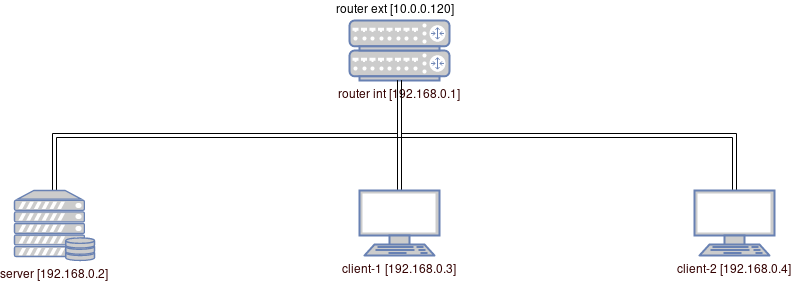
\includegraphics[scale=0.5]{./bilder/tddi41-overview.png}
  \caption{Överblick av noderna i TDDI41}
\end{figure}

Bilden är inte helt rättvisande då den refererar till interna ip-adresser (nätmask /24), 
men det är något vi inte bryr oss nämnvärt vid i det här fallet. Våra exempel kommer även
att förenkla det hela än mer och endast se till det inre nätet. Ett alternativt sätt att
se på det hela är att vi skulle använda enheten \texttt{router} som den maskin vi pushar
våra konfigurationer på. Anledningen till denna förenkling är för att fokusera på och 
tydliggöra själva Ansible-delen snarare än att lösa hela labbserien.
Vi kommer även förutsätta att vi har satt IP-adresser på maskinerna innan vi börjar med Ansible.

Enheten \texttt{router} är en maskin med dubbla nätverkskort (vi bortser från detta här som sagt) som,
precis som namnet antyder, agerar gateway till det inre nätverket samt ntp-server.
Enheten \texttt{server} är en maskin som agerar fillagring, autentiseringsserver, eventuell mailserver, med mera.
Enheterna \texttt{client-\emph{n}} är i det här avseendet identiska sånär som på namn och ip och
är huvudsakligen till för att skala upp miljön.

\section{Hur vi använder Ansible}
När vi vill pusha ändringar till våra noder kan vi använda två olika kommandon: \texttt{ansible} samt \texttt{ansible-playbook}.

Kommandot \texttt{ansible} är det råa kommandot där vi måste specifiera vilka moduler etc. vi skall använda, vilket kan användas för att exempelvis kolla att våra noder är uppe eller för att se variabler som samlas in från en nod. Vi återkommer till detta.

Kommandot \texttt{ansible-playbook} är det vi huvudsakligen kommer att använda oss utav när vi faktiskt pushar ändringar. Det kör då en specifik playbook som anger på vilka noder vad ska köras. Som vi kommer se kan vi göra många justeringar på många system samtidigt med hjälp av dessa playbooks.

\subsection{Vad händer vid en körning}
Om vi ser till vad som händer när vi kör en playbook så händer enkelt sett följande:
Vi ansluter via SSH till noden, skickar över de moduler tillsammans med variabler för hur dessa ska köras samt när, kör en modul som inhämtar körinformation i form av variabler från noden för att (eventuellt) använda dessa variabler tillsammans med de vi skickat med. Till sist kör vi då det script vi skickat över som använder överskickade moduler för att göra förändringarna på noden, och så skickar vi tillbaka körinformation till styrenheten som skriver ut hur det gick på skärmen.

Komplicerat? Ja, bakom ridån, men inte användningsmässigt. Låt oss titta vidare.

\section{Ett faktiskt exempel}
Vi kommer senare att gå in på hostfilen, syntaxer och så vidare, men låt oss först ta ett exempel där vi visar hur enkelt ett kommando för att konfigurera alla client-noder:

\texttt{\$ ansible-playbook clients.yml}

Skulle vi dessutom vilja ansluta som en särskild användare, begränsa oss till en enda klient, begränsa de tasks vi 
vill köra till att endast inkludera NTP-konfiguration och dessutom bara testköra (inga förändringar på den faktiska 
noden), då skulle det kunna se ut som följande:

\texttt{\$ ansible-playbook clients.yml -u foouser -k --limit client-1 --tags NTP -C}

Körkommandot kan i stort sett sköta det mesta, men vanligtvis vill vi ställa in så mycket som möjligt i konfigurationsfilerna, dels Ansibles, men även hostspecifika och gruppspecifika, men mer om det under \ref{sec:bestpractices} Best practices.


\chapter{Filer}\label{sec:files}
I det här avsnittet ska vi titta på de vanligaste konfigurationsfilerna samt viss filstruktur i det upplägg vi senare kommer att beröra i \ref{sec:bestpractices} Best practices.
\section{/etc/ansible}
Under \texttt{/etc/ansible} finner vi systemkonfiguration för styrsystemet samt globalt tillgängliga inventories, roles etc. Vi kommer dock inte att använda mer än \texttt{ansible.cfg} och \texttt{hosts} på en global nivå.
\subsection{ansible.cfg}
Generellt behöver inte den här filen modifieras, men det finns vissa saker som kan vara av intresse även på
en nybörjarnivå.

\texttt{remote\_user} ger oss möjligheten att ansluta med en specifik användare. Vi kommer att beröra detta mer
under best practices.

\texttt{log\_path} kan vara bra att sätta till en lämplig sökväg (ex. \texttt{/var/log/ansible.log}) för att aktivera loggning..

\texttt{vault\_password\_file} ger möjligheten att ange en sökväg för en så kallad 'vault file' - en krypterad fil 
där man kan spara variabler man inte vill ha liggande för allmän åskådan. En sådan fil kan även åkallas på commandline med \texttt{--vault-password-file}.

\texttt{ansible\_managed} är en variabel med samma namn. Denna brukar användas i konfigurationsfiler för att
markera att dessa är konfigurationsstyrda och således inte bör ändras direkt på systemet då dessa ändringar förr 
eller senare kommer att skrivas över.

\texttt{nocows} styr kor. Rekommenderas att sätta till '1' om man inte hyser bovina läggningar.

\subsection{hosts}
\texttt{/etc/ansible/hosts} är den globala host-listan (inventory). Man kan (och eventuellt bör, beroende på miljön i helhet) använda separata hosts-filer och åkalla dessa på kommandoraden.

Inventories är vanligen skrivna i ett init-liknande format, men kan i senare versioner av Ansible även
vara i YAML-format. Vi kommer här att använda det klassiska. Vi kommer att ta vårat exempel från TDDI41 för att
visa hur en sådan kan se ut.

Det vi ser är en enkel enumrering av noderna där vi ger dem funktionella grupperingar (första blocket) där vi
kopplar ihop IP-adresser till dessa grupperingar. Vi skulle lika gärna kunna använda domännamn bör dock sägas, och
skulle vi ha ännu fler noder skulle vi kunna fortsätta lista dessa under grupperingarna. För att demonstrera detta
listar vi även ett subset inaktiva (utkommenterade) clients som inte är aktuella än.

Värt att notera är även att vi kan använda ranges (:). I det här fallet har vi gett ett spann IP-adresser, men skulle vi ha använt oss utav domännamn skulle vi även ha kunnat använda oss av ranges i dessa, exempelvis \texttt{client-[1:2]}

\lstset{language=sh}
\begin{lstlisting}[frame=single]
### BOF ###
## /etc/ansible/hosts
#
## Enumerating nodes

[gateway]
192.168.0.1

[server]
192.168.0.2

[clients]
192.168.0.[3:4]
#192.168.1.[1:50]

## Groupings

[internal:children]
gateway
server
clients

[authnodes:children]
server
clients
### EOF ###
\end{lstlisting}



\chapter{Best practices}\label{sec:bestpractices}
``Best practice'' är ett begrepp som alla har en bild utav vad det innebär inom ens eget område.
Tyvärr är det i stort sett aldrig är så att det finns en enhetlig bild inom varje område, sällan ens
på varje arbetsplats, eller ens mellan team på samma arbetsplats.

När det gäller systemadministration så är det givetvis likadant, och det viktigaste är i sedvanlig ordning dokumentation.
Har man en god dokumentation så kan resten lösas med resurser. Ansible är inte avsett att vara ett dokumentationsverktyg,
men det kan utgöra ett utmärkt komplement till exempelvis en wiki.

Men, det här är inte en guide till systemadministration eller dokumentation, det är en guide till Ansible, så låt 
oss fokusera på detta.

Best practice är till viss del beroende på hur vad man använder Ansible till och hur stora och varierade miljöer
man har. Den här guiden försöker främst hålla ett scenario tanken där vi har en varierad miljö med olika 
linuxdistributioner och där vi samtidigt söker en skalbarhet. Att hantera en eller ett par maskiner klarar man utan
att blanda in exempelvis Ansible (även om det är praktiskt att kunna rulla om maskiner smidigt), men att hålla
tiotals, hundratals, eller till och med tusentals klienter i ordning på ett enhetligt sätt kräver verktyg, och varje
miljö börjar med en första maskin.

Att använda någon form av versionshantering är att se som lite av ett måste när samarbete mellan administratörer
förekommer, och även en automatiseringskedja när miljön växer. Det är dock två faktorer vi inte kommer att beröra
här då det är utanför denna guides ``scope'', men möjligheterna finns.

\section{Filstruktur}
En tydlig filstruktur hjälper skalbarhet, läsbarhet och även implementation av versionshantering (ex. Git). Det 
finns flera olika modeller som är bra, men här lyfts bara en av den enkla anledningen att det är en modell 
undertecknad själv har använt framgångsrikt och för att omfattningen av denna guide skall hållas begränsad. Den 
är en av de modeller som rekommenderas av RedHat, så det är inget hemkok på något sätt. Vi börjar med att illustrera
den:

\begin{verbatim}
./
  hosts                   # global inventory file
  
  group_vars/
    <groupname>           # variables for groups
  host_vars/
    <hostname>            # variables for specific systems
  
  library/                # custom modules
  filter_plugins/         # custom filter plugins
  
  roles/                  
    common/               # this hierarchy represents a "role"
        tasks/            #
            main.yml      #  <-- tasks file can include smaller files if warranted
        handlers/         #
            main.yml      #  <-- handlers file
        templates/        #  <-- files for use with the template resource
            ntp.conf.j2   #  <------- templates end in .j2
        files/            #
            bar.txt       #  <-- files for use with the copy resource
            foo.sh        #  <-- script files for use with the script resource
        vars/             #
            main.yml      #  <-- variables associated with this role
        defaults/         #
            main.yml      #  <-- default lower priority variables for this role
        meta/             #
            main.yml      #  <-- role dependencies

\end{verbatim}


\chapter{Playbooks}\label{sec:playbooks}
En playbook skrivs i YAML-format. Låt inte detta avskräcka om du aldrig skrivit en rad YAML tidigare, för det är
rätt så lätt att lära sig. Det som är viktigt att komma ihåg är att indentering spelar roll. Det spelar ingen roll 
om du använder mellanslag eller tabbar, men "nivåerna" spelar roll.

En playbook innehåller ``plays'' (den som är bekant med amerikansk fotboll känner igen termerna). 
En play är en mappning av ``tasks'' som skall utföras på en grupp hostar i syfte att nå ett bestämt och känt state.

Vi börjar med ett litet exempel:

\begin{verbatim}
---
- hosts: all
  tasks:
    - name: "Ensure NTP package is installed"
      package:
        name: ntp
        state: present
      notify:
        - restart ntp

  handlers:
    - name: restart ntp
      service:
        name: ntpd
        state: restarted
...
\end{verbatim}

Vi börjar här med en filstart \texttt{---} följt av att vi bestämmer att påföljande tasks skall köras på \texttt{all}, vilket är ett nyckelord och inkluderar samtliga noder i inventoryt. Även \texttt{*} kan användas, och kan användas som wildcard i exempelvis IP-adresser. Vi kan även ange en specifik host eller gruppering. Skulle vi vilja exkludera går även det att göra, precis som vi kan göra en host required, exempelvis:

\verb+webservers:!{{excluded}}:&{{required}}+

Rad tre påbörjar en lista med tasks, och på rad fyra börjar den första (och enda) genom att vi ger den ett \texttt{name}.
Detta är inget som behövs, som tidigare nämnts, men det bör ges. Därefter säger vi att vi skall använda modulen 
\texttt{package} för att säkerställa att paketet \texttt{ntp} är installerat (\texttt{present}). Om denna task körs
och åstadkommer någon förändring på systemet (i det här fallet, installeras) så säger vi till Ansible att anropa en
handler (\texttt{notify}).

Sedan har vi själv handlern, vilket i princip är en task, men den körs endast en gång per play, och endast om den 
anropats till följd av en notify. Hade vi haft en task till som exempelvis justerat en konfigurationsfil med samma notify så hade denna handler körs en (1) gång, även om vi både installerat paketet och justerat konfigurationsfilen, men inte körts om vi direkt efter kört samma playbook en gång till eftersom paketet då varit installerat och konfigurationsfilen varit oförändrad.

Handlern \texttt{restart ntp} i det här fallet använder modulen \texttt{service} för att starta om tjänsten \texttt{ntpd}. Kort om \texttt{service}-modulen kan nämnas att den stödjer de flesta system för daemons som används idag.

Om du inte riktigt greppat konceptet med moduler så är det inget att oroa sig för. Vi kommer att gå in djupare på det vad det lider.

\section{Användare}
Att hålla koll på vilken användare som används på styrenheten likväl som hostarna är ett måste. Vi kan inte anta att
alla som ska köra en playbook har root-access eller ens bör ha. Samtidigt kommer många saker att kräva förhöjda 
rättigheter för att utföras. Likaså kanske inte det konto som används på styrenheten ens finns på (alla) hostarna.

Vi nämnde \texttt{remote\_user} i config-filen tidigare, vilket möjliggör att vi exempelvis kan sätta \texttt{root}
som ``default'', men det är inte alltid att föredra det heller. Best practice vore i stället att ha ett lokalt 
servicekonto på varje nod -- låt oss kalla det för \texttt{ansacc} (kort för ansible account) -- med ssh-nyckel.
Detta servicekonto ges sedan sudorättigheter att bli \texttt{root} (företrädesvis med lösenord vilket sparas i en
vault-fil, men det är överkurs). Därefter kan vi använda oss utav \texttt{become: yes} för att eskalera rättigheterna där det behövs.

\begin{verbatim}
---
- hosts: all
  become: yes
  tasks:
    [...]
...
\end{verbatim}

\section{Taggar}
Inte sällan tar det tid att köra långa plays, inte minst när vi börjar jobba med roles, och då är det onödigt att
behöva mata genom hela batteriet om vi bara vill ändra en enskild sak. Då blir det lätt att man undviker 
konfigurationsstyrning och sedan faller hela poängen. Därför är taggar bra att använda i tasks för att på så sätt
kunna begränsa de tasks som ska köras i en playbook. Så för att kunna urskilja NTP-relaterade prylar genom vårat 
grundläggande körexempel tidigare ger vi vår playbook taggen NTP:

\begin{verbatim}
---
- hosts: all
  tasks:
    - name: "Ensure NTP package is installed"
      package:
        name: ntp
        state: present
      tags: NTP
      notify:
        - restart ntp

  handlers:
    - name: restart ntp
      service:
        name: ntpd
        state: restarted
      tags: NTP
...
\end{verbatim}

Varje task kan ges flera taggar i en kommaseparerad lista (OR:ad, så en räcker för att aktivera).

\section{Importera task lists och variabelfiler}
Ansible tillåter playbooks och task lists att importera andra filer med task lists som kommer att köras in-line. Detta kan
vara smidigt inte minst i roles som ska stödja olika distributioner som kräver olika steg från varandra. Likaså
kan separata filer med variabler.

Dessa två actions är:
\texttt{include\_tasks} och \texttt{include\_vars}. Även \texttt{import\_tasks} och \texttt{import\_vars} kan
användas, med skillnaden att \texttt{import*} preprocessas när playbooken parsas, medan \texttt{include*} processas
när de stöts på under körningen.

\section{Variabler}
Variabler är det som gör Ansible till mer än bara en exekverare av statiska skript.
Variabelnamn startar med en bokstav och kan innehålla [A-Za-z0-9\_]. Märk väl att bindestreck inte är tillåtna.
Variabler är inte helt triviala, och jag rekommenderar starkt att läsa \href{https://docs.ansible.com/ansible/2.6/user_guide/playbooks_variables.html}{\em Ansibles dokumentation} i ämnet. Fortsatt kommer det här dokumentet att förutsätta att läsaren själv slår upp denna dokumentation när tveksamhet råder.


\chapter{Roles}\label{sec:roles}
% TODO: I playbooks - lägg till import av andra playbooks
Roles -- roller -- är egentligen inte mycket annat än playbooks som inte är hostbundna; m.a.o. en template.

Som den uppmärksamme såg tidigare bygger en role på en katalogstruktur där den enda obligatoriska katalogen och 
filen är \texttt{./roles/rolename/tasks/main.yml}. Den filen är i princip en reducerad playbook där vi brutit ut
tasks till en separat fil. Har vi handlers bryter vi ut dem till \texttt{handlers/main.yml}.

Att följa given katalogstruktur gör även att Ansible själv hittar exempelvis handlers, variabler etc.

\section{Variabler i roles}
Variabler i roller kan användas i flera lager med olika prioritet. Lägst prioritet har variabler i 
\texttt{defaults/main.yml}. Dessa kan i sin tur skrivas över av importerade variabler. Fördelen med att ha 
defaults är givetvis att vi inte kommer få problem vid körning på grund av att en variabel inte är deklarerad.
Således bör alla egna variabler vara deklarerade i \texttt{defaults/main.yml}.

Exempelvis skulle våran tidigare NTP-playbook kunna vara en roll som ser ut som följande i role-form med paketnamnet som variabel (vilket är overkill för TDDI41, men vilket vore smidigt i en distromixad miljö):

\begin{verbatim}
### ./roles/ntp/tasks/main.yml ###
---
- name: "Ensure NTP package is installed"
  package:
    name: '{{ ntp_package }}'
    state: present
  tags: NTP
  notify:
    - restart ntp
...

### ./roles/ntp/handlers/main.yml ###
---
- name: restart ntp
  service:
    name: ntpd
    state: restarted
  tags: NTP
...

### ./roles/ntp/defaults/main.yml ###
---
ntp_package: ntp
ntp_server: false
...
\end{verbatim}

\section{Filöverföring}
Att föra över filer från styrhost till nod är inte det vanligaste, men det kan behöva göras emellanåt. Filer
lagrade under \texttt{files} är lättrefererade eftersom Ansible kommer att söka där först och främst.
Främst används dessa av \texttt{copy}-modulen vilken vi inte kommer att beröra här, men återigen är Ansibles
dokumentation lättfunnen.

Vad som är mer intressant är \texttt{templates} där vi kan lagra konfigurationsfilsmallar (vilket vi kommer att 
beröra). Detta är mallar som kan vara scriptade för att dynamiskt kunna anpassa sig utifrån variabler (antingen
insamlade från noden, eller inskickade vid körning) och på så sätt på ett smidigt sätt konfigurera en host.

\section{Roles i playbooks}
För att använda roles måste vi koppla dessa till noder i en playbook. Den uppmärksamme lade även märke till
variabeln \texttt{ntp\_server} ovan. Vi kommer senare att visa hur denna kan användas i en template för att
låta en fil konfigurera både en ntp-server och ntp-klienter. Vi förutsätter dock här att det redan är med i 
tasks-listan och att templaten är på plats, när vi nu visar på hur en playbook som nyttjar detta kan se ut:

\begin{verbatim}
### ./playbook.yml
---
- hosts: gateway
  become: yes
  roles:
    - { role: ntp, tags: ["NTP","gateway"], ntp_server: true }

# Här ser vi en alternativ formattering som är motsvarande den ovan. 
# Vilken man vill använda är en smaksak.

- hosts: authnodes
  become: yes
  roles:
    - role: ntp
      tags: NTP,authnodes
      ntp_server: false
\end{verbatim}

Den uppmärksamme har säkerligen även ifrågasatt varför vi har med \texttt{ntp\_server: false} när den är deklarerad
som \texttt{false} i \texttt{defaults/main.yml}. Det är en god iakttagelse, och den enda anledningen är för att 
visa på de olika formatteringarna. Det skadar givetvis inte att skicka med den, och det skulle kunna vara att 
rekommendera utifall att vi av någon anledning skulle få för oss att ändra default-värdet vid senare tillfälle.


\chapter{Modules}\label{sec:modules}
Den stora bredd på välskrivna moduler som skeppas med Ansible är vad som separerar Ansible från alternativen.
Den här guiden är på intet sätt avsedd att omfatta ens en bråkdel av modulerna, men vi kommer att nämna de
vanligaste och mest grundläggande för att "komma igång". Inte heller tas allting upp som kan göras med respektive
modul. Därav kan du härmed se dig permanent refererad till Ansibles dokumentation. Även jag som jobbar med
Ansible har oftast en eller flera tabbar med dokumentation för olika moduler uppe i min webbläsare. 
Dokumentationen finns där av en anledning -- att användas. Att memorera annat än namnen på de allra vanligaste är
ett slöseri med tid i de flesta fall.

Varje modulsektion nedan kommer med ett mer eller mindre grundläggande exempel. I de fall det är mer än minimala
exempel så beror det på att jag antingen vill belysa en kraftfull användning av modulen eller att jag vill introducera något koncept.

\section{package}
Packagemodulen används för att installera paket med pakethanterare. De flesta pakethanterare har en egen modul som
är betydligt kraftfullare än \texttt{package}, men i nio av tio fall räcker denna modul mer än väl. Fördelen är att
vi inte behöver fundera på om systemet använder dpkg, yum, pacman eller whatever, vi behöver bara bry oss om vad 
paketet vi vill hantera heter. Ofta har paket samma namn mellan distar, men det kan skilja sig åt och då behöver
man täcka upp för det (se många av mina ansible-role-repon för exempel på detta). Betänk att pakethanterare ofta
behöver root-privilegier.

Modulen har och behöver två parametrar:
\texttt{name} ger namnet på det paket som ska hanteras.

\texttt{state} bestämmer om paketet i fråga ska vara installerat (\texttt{present}) eller inte (\texttt{absent}). De
flesta underliggande moduler stödjer även (\texttt{latest}).

\begin{verbatim}
- name: Install SELINUX libs if needed
  when: ansible_selinux and ansible_selinux.status == 'enabled'
  become: True
  package:
    name: "{{ item }}"
  with_items:
    - libselinux-python
    - policycoreutils-python
\end{verbatim}


\section{template}
Vi kommer att titta närmare på hur vi bygger templates senare, men till en början ska vi se hur vi använder modulen.

\begin{verbatim}
- name: configure ntp (ntpd)
  when: ( ansible_os_family == 'RedHat' and ansible_distribution_major_version == '6') or
        systemd_ntpd.stat.islnk is defined
  notify: restart ntp
  become: true
  template:
    src: "ntp.conf_{{ ansible_os_family }}{{ ansible_distribution_major_version }}.j2"
    dest: /etc/ntp.conf
  tags: NTP
\end{verbatim}

Det här är en task som bjuder på lite variabelanvändning (bara för demonstration av variabler samt konditionell 
användning, så \texttt{when}-delen är inte relevant för modulen i sig). Men, om vi ser till de modulrelevanta 
raderna så ser vi följande:

\begin{verbatim}
- name: configure ntp (ntpd)
  template:
    src: "ntp.conf.j2"
    dest: /etc/ntp.conf
\end{verbatim}

Vi har en template, \texttt{templates/ntp.conf.j2} på styrsystemet som vi använder för att konfigurera \texttt{/etc/ntp.conf} på noderna. Exemplet ovan är minimalt, men det finns fler användbara parametrar:

\texttt{backup: yes} skapar en backupfil med timestamp så att du kan återställa originalet om det skulle behövas.

\texttt{validate} erbjuder möjligheten att validera den nya filen med valt kommando innan vi skriver över den gamla.
Sökvägen skickas som \verb+%s+ (se exempel nedan).

Det kan även vara bra att känna till några andra parametrar, nämligen de som styr filrättigheter:

\texttt{owner} anger vilken user som ska ha rättigheter (per default är det den användare som ansible använder, d.v.s. den man ansluter som eller den man eleverar sig till (\texttt{root} i fallet \texttt{become: yes})).

\texttt{group} är som \texttt{owner} men för group.

\texttt{mode} agerar chmod, men har lite egenheter. Den accepterar symbolic mode (ex. \texttt{u+rwx}) och även
oktetter. Använder vi oss av en oktala värden behöver modulen dock veta det genom att vi inleder med 0, alternativt
sätter det inom enkla citattecken, ex. \texttt{0644, 01777} eller \texttt{'644'}. Vi kan även skicka \texttt{preserve} för att bibehålla befintliga rättigheter (endast Ansible 2.6 eller senare.)

Exempel:
\begin{verbatim}
- name: "Update sshd config safely to avoid locking yourself out."
  template:
    src: etc/ssh/sshd_config.j2
    dest: /etc/ssh/sshd_config
    owner: root
    group: root
    mode: '0600'
    validate: /usr/sbin/sshd -t -f %s
    backup: yes
\end{verbatim}

\section{service}
Den här modulen har vi sprungit på tidigare, och den stödjer BSD init, OpenRC, SysV, Solaris SMF, systemd och upstart. De viktigaste parametrarna är:

\texttt{name} - obligatorisk.

\texttt{enabled} - huruvida servicen skall autostarta. Boolean \texttt{yes/no}. Obligatorisk om inte \texttt{state} anges.

\texttt{state} - obligatorisk om inte \texttt{enabled} anges. De båda är inte exklusiva och påverkar inte varandra,
men endera eller båda krävs. Tar argumenten \verb+reloaded/restarted/running/started/stopped+, där de sista två är idempotenta och körs inte om de inte behövs. Märk väl att \verb+reloaded+ kommer att starta servicen om den inte 
är startad redan, oavsett vad init-systemet i fråga gör i vanliga fall.

\section{shell/command}
De här modulerna är i stort sett identiska, men \texttt{shell} kör kommandot i ett eget skall (\texttt{/bin/sh}) på 
aktuell nod. Generellt sett bör \texttt{command} användas.

Modulerna tar in kommandoraden som skall köras direkt efter modulcallen, och oftast vill vi ta ut ett resultat från 
körningen, vilket vi gör genom att tilldela tasken en registrerad variabel:

\begin{verbatim}
- name: return motd to registered variable
  command: cat /etc/motd
  register: mymotd
\end{verbatim}

Parametrar vi vanligen vill använda är \texttt{creates/removes} samt \texttt{chdir}. Sistnämnda ändrar directory alldeles innan kommandot körs, och de förstnämnda kollar huruvida given path existerar, och om den gör/inte gör det så körs kommandot. Att sätta parametern tar inte bort eller skapar filerna i sig, utan utgår från att kommandot skapar dessa.

\section{file}

\section{lineinfile}

\section{stat}

\section{group}

\section{user}


\chapter{Efterord}\label{sec:outro}
Den här guiden skrapar, återigen, bara på ytan av Ansibles fulla potential. Den bör dock ge en smidig väg in i
Ansibles värld, och öppna upp ögonen på läsaren för en helt ny värld (åtminstone om vederbörande aldrig använt
något dylikt verktyg tidigare). Förhoppningsvis kommer läsaren att fortsättningsvis fundera på "hur kan jag lösa
det här med Ansible" snarare än att göra enskilda förändringar på enskilda maskiner om och om igen bara för att 
"det är ju minst lika smidigt att copy-n-paste:a eller tmux:a".

Lycka till och glöm inte en sysadmins ledord: Var lat, och gör det du gör väl så behöver du aldrig göra det igen.


\end{document}
